%%%%%%%%%%%%%%%%%%%%% Reporte %%%%%%%%%%%%%%%%%%%%%
\documentclass[12pt, a4paper]{report}
\usepackage[spanish]{babel}
\usepackage[utf8]{inputenc}
%%%%%%%%%%%%%%%%%%%%% Paquetes %%%%%%%%%%%%%%%%%%%}		
\usepackage{geometry}
\usepackage{graphicx}
\usepackage{amssymb,amsmath,amsthm,amstext,amsfonts}
\usepackage{color}

%%%%%%%%%%%%%%%%%%%% CÓDIGO %%%%%%%%%%%%%%%%%%%%%%
\usepackage{listings}
\usepackage{xcolor}

% Configuración del estilo para código en Python
\lstset{
    language=Python,                    % Cambia el lenguaje a Python
    backgroundcolor=\color{lightgray!20}, % Color de fondo
    basicstyle=\ttfamily\footnotesize,   % Estilo básico del código
    keywordstyle=\color{blue},           % Color de las palabras clave
    commentstyle=\color{green!50!black}, % Color de los comentarios
    stringstyle=\color{red},             % Color de las cadenas de texto
    numbers=left,                        % Mostrar los números de línea a la izquierda
    numberstyle=\tiny\color{gray},       % Estilo de los números de línea
    stepnumber=1,                        % Incremento entre los números de línea
    breaklines=true,                     % Dividir líneas largas automáticamente
    frame=single,                        % Agregar un borde alrededor del código
    captionpos=b,                        % Poner la leyenda (caption) debajo del código
}

%\begin{lstlisting}[caption={Función de nodos}, label={lst:nodos}]
 %% ESCIBE TU CÓDIGO AQUÍ
%\end{lstlisting}
%%%%%%%%%%%%%%%%%%%%%%%%%%%%%%%%%%%%%%%%%%%%%%%%%%%%%%%%%%%%%%%

\setlength{\parindent}{0pt}

\graphicspath{ {Img/} }

% Colors for the hyperref package
\definecolor{urlcolor}{rgb}{0,.145,.698}
\definecolor{linkcolor}{rgb}{.71,0.21,0.01}
\definecolor{citecolor}{rgb}{.12,.54,.11}

%%%%%%%%%%%% NEW THEOREM %%%%%%%%%%%%%%%%%
\providecommand{\abs}[1]{\lvert#1\rvert}
\newtheorem{definition}{Definición}
\newtheorem{proposition}{Proposición}
\newtheorem{remark}{Observación}
\newtheorem{notation}{Notación}
\newtheorem{lemma}{Lema}
\newtheorem{theorem}{Teorema}
\newtheorem{example}{Ejemplo}
%%%%%%%%%%%%%%%%%%%%%%%%%%%%%%%%%%%%%%%%%%%%%%%%%

\title{Tesis de posgrado.}
\author{Eduardo Ortiz Romero}

%%%%%%%%%%%%%%%%%%%%%%%%%%%%%%%%%%%%%%%%%%%%%%%

\begin{document}
\maketitle
\tableofcontents

\chapter{Introducción}

\section{Problema 16 de Hilbert}
En 1900, el matemático alemán David Hilbert presentó una lista de 23 problemas abiertos en el Congreso Internacional de Matemáticos en París. Estos problemas de diversas áreas de las matemáticas, se convirtieron en una guía fundamental para la investigación matemática del siglo XX y, en muchos casos, aún siguen desafiando a la comunidad científica.\\

El \textbf{problema 16 de Hilbert}  forma parte de esta lista y está dividido en dos partes principales. Ambas se centran en el análisis geométrico y topológico de curvas algebraicas y sistemas dinámicos polinomiales en el plano:

\begin{enumerate}
	\item \textbf{Primera parte:} Clasificar las disposiciones topológicas posibles de las curvas algebraicas planas reales de grado $n$. Este problema está relacionado con la geometría algebraica real y la topología.
	\item \textbf{Segunda parte:} Estudiar los sistemas dinámicos definidos por campos vectoriales polinomiales en el plano, y en particular, determinar el número máximo y la disposición de los ciclos límite que estos sistemas pueden tener.
\end{enumerate}

La segunda parte del problema 16 de Hilbert aborda una cuestión fundamental en la teoría de sistemas dinámicos: la existencia, finitud y disposición de ciclos límite en sistemas de ecuaciones diferenciales polinomiales. Un ciclo límite es una órbita cerrada aislada en el espacio de fases, alrededor de la cual las trayectorias vecinas convergen o divergen en espiral hacia adentro o hacia afuera.\\

Consideremos el sistema de ecuaciones  en el plano polinomial de grado $n$:

\begin{equation}
	x'=P\left(x,y\right)\text{, }\text{  }y'=Q\left(x,y\right)
\end{equation}
donde $P\left(x,y\right)$ y $Q\left(x,y\right)$ son polinomios de grado a lo más $n$. El problema consiste en responder las siguientes preguntas:
\begin{enumerate}
	\item ¿Cuántos ciclos límite puede tener un sistema polinómico de grado $n$?
	\item ¿Cómo están distribuidos estos ciclos límite en el plano?
\end{enumerate}

¿Sencillo? pues no, la respuesta sigue siendo desconocida para $n>1$.

\section{Resultados relevantes sobre la existencia de ciclos límite}

Tenemos algunos resultados significativos como la conjetura de Dulac, que establece que para cualquier n, el número de ciclos límite de un sistema polinómico de grado $n$ es finito, sin embargo esto es una conjetura y aún no se ha probado.  Analicemos los resultados más relevantes conocidos hasta la fecha acerca de la existencia de ciclos límite en el contexto del problema 16 de Hilbert.

\begin{enumerate}
	\item \textbf{Teorema de Poincaré- Bendixón} Establece las condiciones suficientes para la existencia de ciclos límite en sistemas planares. Este teorema será central en el análisis de esta tésis.
	
	\item \textbf{Conjetura de Finitud de Dulac}
	\begin{itemize}
		\item 	En 1923, Henri Dulac planteó la conjetura de que el número de ciclos límite de un sistema polinómico de grado $n$  en el plano es finito. 
		\item Jean Écalle y Yulij Il'yashenko, de forma independiente en 1991, probaron la conjetura de finitud de Dulac. Demostraron que para sistemas polinómicos planos, el número de ciclos límite es finito. Este resultado es significativo porque confirma que, aunque no se conoce el número máximo exacto de ciclos límite para cada grado $n$
		, al menos se sabe que este número es finito.
	\end{itemize}

	\item \textbf{Sistemas Polinomiales de Bajo Grado}
	\begin{itemize}
		\item 	Los sistemas lineales en el plano ($n=1$) no poseen ciclos límite. Toda órbita es o bien una trayectoria hacia o desde un punto de equilibrio, o una familia de órbitas paralelas.

		\item Hasta ahora, el máximo número de ciclos límite conocidos en sistemas cuadráticos es $4$, pero no se ha probado que este sea el número máximo posible. Nikolai Bautin en 1939 analizó las bifurcaciones en sistemas cuadráticos y encontró condiciones para la aparición de ciclos límite pequeños alrededor de puntos singulares.
	\end{itemize}

	\item \textbf{Teoría de Bifurcaciones y Ciclos Límite}
	La teoría de bifurcaciones ha sido una herramienta clave en el estudio de los ciclos límite.
	\begin{itemize}
		\item \textbf{Bifurcación de Hopf}: Describe cómo un ciclo límite puede emerger o desaparecer al variar un parámetro en el sistema.
		\item \textbf{Ciclos Límite Múltiples}: Investigaciones han mostrado que es posible tener múltiples ciclos límite que rodean puntos singulares o áreas sin puntos singulares.
	\end{itemize}
	\item \textbf{Métodos Analíticos y Geométricos}
	\begin{itemize}
		\item 	\textbf{Función de Dulac}
		Dulac introdujo una función auxiliar (ahora conocida como función de Dulac) para estudiar la no existencia de ciclos límite en ciertas regiones.
		\item \textbf{Teoría de Hilbert-Poincaré}
		Variedades Algebraicas: Se utilizan herramientas de geometría algebraica para entender las propiedades globales de los sistemas polinómicos.
		
		\item \textbf{Análisis de Singularidades}: El estudio de puntos críticos y sus tipos es esencial para comprender la dinámica local y global.
	\end{itemize}

	\item \textbf{Métodos de Perturbación}
	Se han utilizado métodos de perturbación y teoría de promediación para estudiar la aparición de ciclos límite en sistemas cercanos a sistemas integrables.
	\item \textbf{Teoría de Foliaciones}
	El estudio de foliaciones en el plano ha proporcionado nuevas perspectivas sobre la estructura de las órbitas y la posible existencia de ciclos límite.

\end{enumerate}

\section{Problemas clásico de ciclos límite}

Los sistemas dinámicos ofrecen la posibilidad de explorar comportamientos oscilatorios que son inherentes a muchos procesos biológicos, químicos y físicos. A continuación, se presentan varios ejemplos donde los ciclos límite desempeñan un papel central.

\newpage

\begin{itemize}
	\item \textbf{Oscilador de Van der Pol}\\
	
	El oscilador de Van der Pol es un ejemplo clásico de un sistema no lineal que exhibe ciclos límite. Originalmente desarrollado para modelar circuitos eléctricos con tubos de vacío, este sistema también describe fenómenos auto-oscilatorios en ingeniería y biología.
	\begin{equation}
		x''-\mu \left(1-x^2\right)x'+x=0
	\end{equation}
	donde $\mu$ es el coeficiente de amortiguamiento.  A medida que $\mu$ aumenta, el sistema muestra un ciclo límite estable que corresponde a una oscilación sostenida. Este comportamiento es crucial para entender dispositivos electrónicos oscilatorios y ciertos ritmos biológicos.

	\begin{figure}[h]
		\centering
		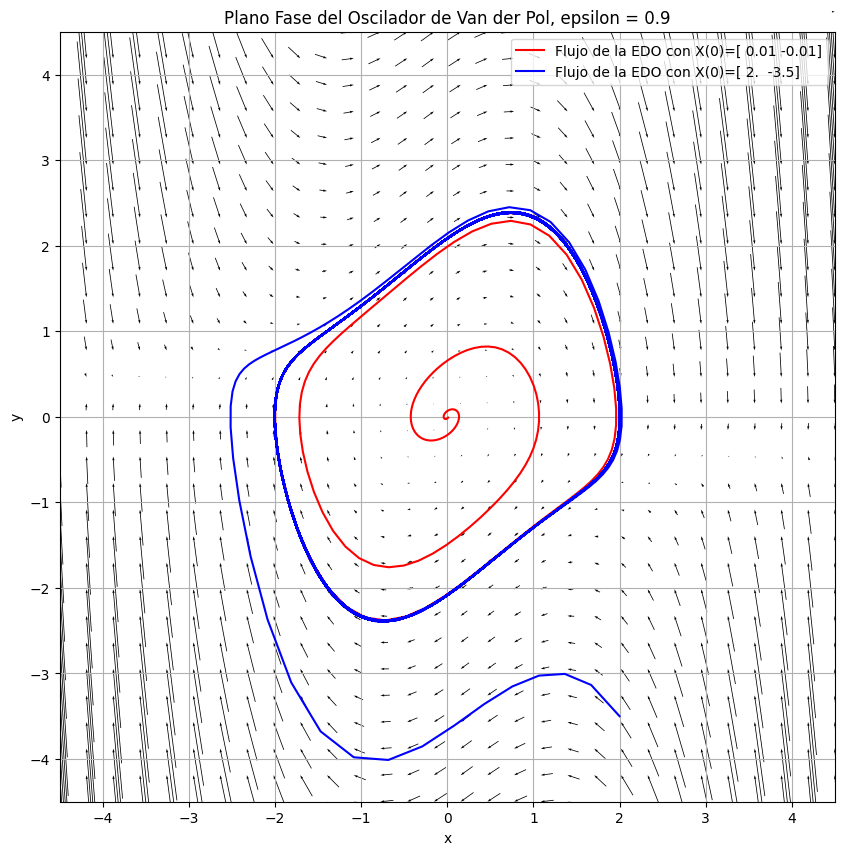
\includegraphics[width=11cm]{introVanderPol.png}
		\caption{Plano fase del Oscilador de Van der Pol}
	\end{figure}

	\newpage

	\item \textbf{Ecuación de Rayleigh}\\
	
	La ecuación de Rayleigh modela el comportamiento de ciertos sistemas mecánicos y fluidos sometidos a fuerzas periódicas. Es similar al oscilador de Van der Pol.
	\begin{equation}
		x''+x=\epsilon\left(1-x'^2\right)x'
	\end{equation}
	donde $\epsilon$ controla la intensidad de la fuerza. Los ciclos límite en este modelo describen el fenómeno de resonancia mecánica y son fundamentales para el diseño de sistemas que requieren estabilidad en las oscilaciones, como los amortiguadores en vehículos.

	\begin{figure}[h]
		\centering
		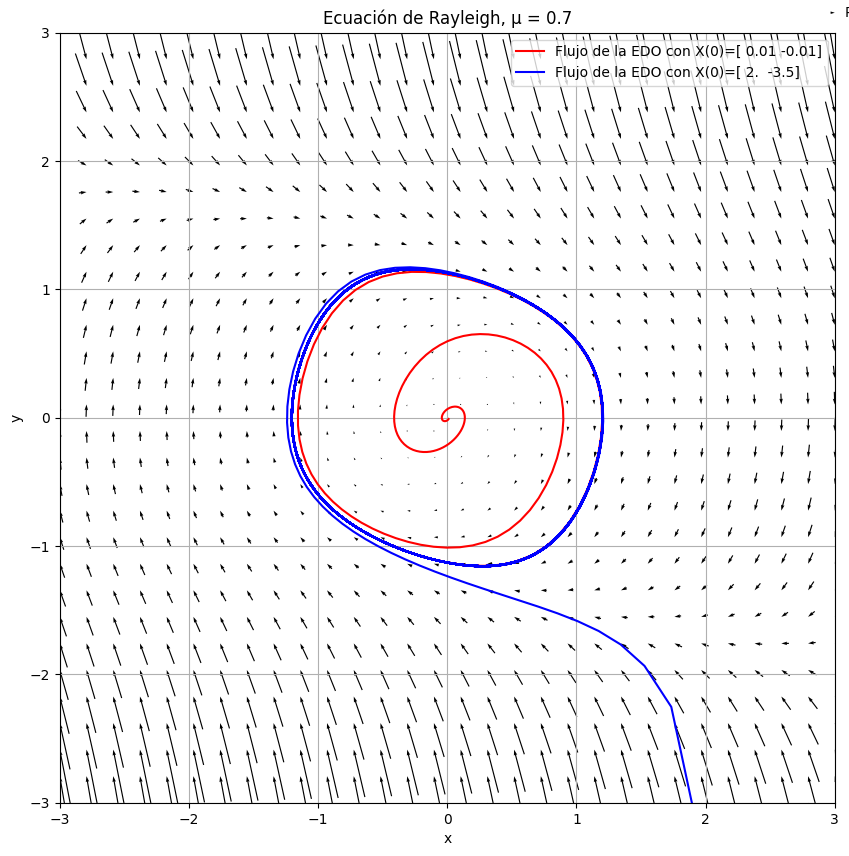
\includegraphics[width=13cm]{introRayleigh.png}
		\caption{Plano fase de la ecuación de Rayleigh}
	\end{figure}

	\newpage

	\item \textbf{Modelo de Fitz Hugh-Nagumo}\\
	
	Este modelo es una simplificación del modelo de Hodgkin-Huxley y se utiliza para describir la activación y desactivación de las neuronas. 
	\begin{equation}
		\begin{matrix}
			v'=v-\frac{v^3}{3}-w+I\\
			w'=\epsilon\left(v+a-bw\right)
		\end{matrix}
	\end{equation}
	donde $v$ representa el potencial de membrana, $w$ es una variable de recuperación, e $I$ es un término de corriente externa. Los ciclos límite en este sistema modelan los potenciales de acción neuronal, esenciales para entender el procesamiento de la información en el cerebro.\\

	\begin{figure}[h]
		\centering
		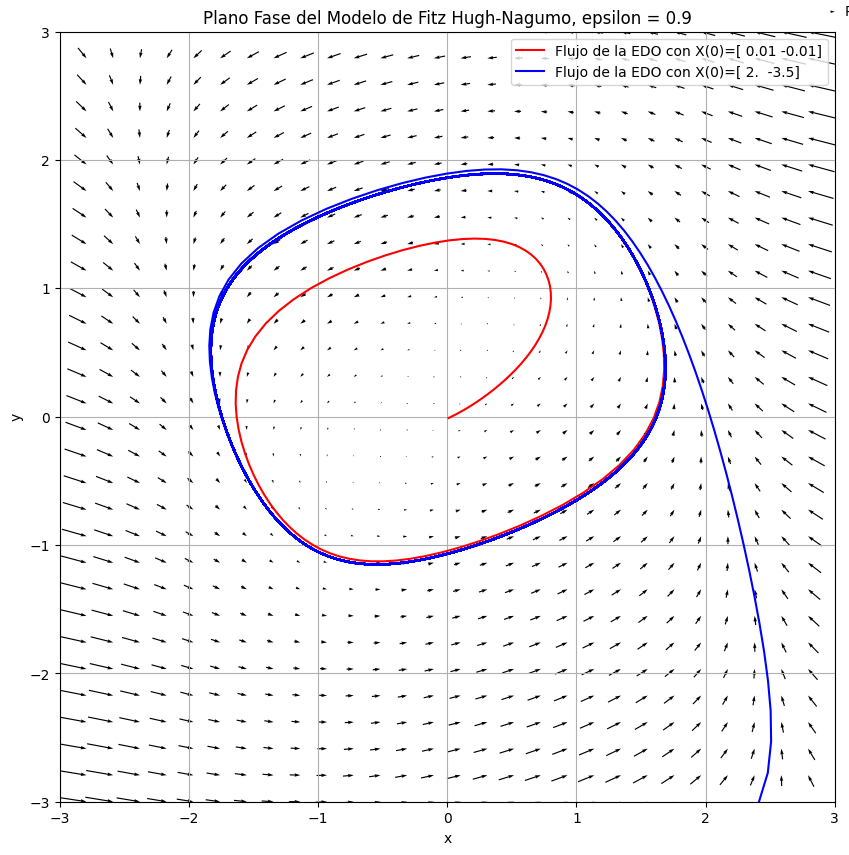
\includegraphics[width=12cm]{introFitz.png}
		\caption{Plano fase del Modelo de Fitz Hugh-Nagumo}
	\end{figure}

	\newpage

	\item \textbf{Reacciones Químicas Oscilatorias}\\
	
	Un ejemplo destacado es la reacción de Belousov-Zhabotinsky, que es un tipo de reacción química que muestra oscilaciones temporales en la concentración de sus reactivos. Aunque su modelado exacto requiere ecuaciones más complejas, sistemas simplificados que muestran ciclos límite pueden ayudar a comprender la dinámica subyacente de estas reacciones oscilatorias.
\end{itemize}
Más adelante vamos desarrollar estos modelos a profundidad.
\newpage


\chapter{Preliminares}

\section{Coordenadas polares}

Cuando realizamos un cambio de coordenadas cartesianas $(x,y)$ a coordenadas polares $(r,\theta)$ en un sistema de ecuaciones diferenciales en el plano, no solo transformamos el aspecto algebraico del sistema, sino que también ganamos una interpretación geométrica más natural de la dinámica. Este cambio tiene varias implicaciones importantes: 

\begin{enumerate}
	\item \textbf{Descomposición del movimiento en componentes radiales y angulares:}
	En coordenadas cartesianas, las trayectorias del sistema se describen por $(x(t),y(t))$, lo cual puede dificultar la interpretación de cómo cambia la distancia al origen o la dirección del movimiento.\\

	Al pasar a coordenadas polares:
	\begin{equation}\label{eq:xpolar}
		x=r\cos(\theta)
	\end{equation}
	\begin{equation}\label{eq:ypolar}
		y=r\sin(\theta)
	\end{equation}
	las variables pasan a ser:
	\begin{itemize}
		\item $r(t)$, la distancia del punto en movimiento con respecto al origen.
		\item $\theta(t)$, el ángulo que determina la orientación del punto con respecto al eje $x$.
	\end{itemize}
	
	Esto nos permite analizar la dinámica en términos de:
	\begin{itemize}
		\item \textbf{Crecimiento o decrecimiento radial:} si $r'$ es positiva, el sistema se aleja del origen; si es negativa, se acerca.
		\item \textbf{Rotación angular:} $\theta'$  indica con qué rapidez y en qué sentido gira la solución alrededor del origen.
	\end{itemize}
	\item \textbf{Interpretación de estabilidad y ciclos límite:}
	Muchos sistemas dinámicos en el plano poseen soluciones periódicas (ciclos límite) o puntos de equilibrio. En coordenadas cartesianas, identificar la naturaleza de estos objetos puede ser menos intuitivo.\\

	En coordenadas polares:

	\begin{itemize}
		\item Un \textbf{punto de equilibrio en el origen} (es decir, $r=0$) se interpreta geométricamente como un estado estacionario donde el sistema ni se expande ni gira, o bien la dinámica angular se vuelve irrelevante.
		\item Un \textbf{ciclo límite} se ve naturalmente como una condición donde el radio $r$ se hace constante en el tiempo ($r'=0$) y el ángulo $\theta$ cambia a una velocidad constante ($\theta'\neq0$). Esto describe una órbita cerrada alrededor del origen. Geométricamente, es una solución periódica establecida por una distancia fija al origen y una rotación estable alrededor de él.
	\end{itemize}
	\item \textbf{Simplicidad para el análisis de oscilaciones y bifurcaciones:}
	Muchos fenómenos oscilatorios (como el oscilador de Van der Pol o sistemas en torno a centros y focos) adquieren una descripción más simple al observar el comportamiento radial y angular. Por ejemplo, la aparición de un ciclo límite a partir de un punto de equilibrio a través de una bifurcación de Hopf es más sencilla de describir en polares, ya que el límite cíclico se interpreta directamente como la estabilización de una órbita en $r$.
	\item \textbf{Separación de efectos radiales y angulares:}
	Algunas perturbaciones o forzamientos del sistema afectan más claramente el componente radial (por ejemplo, forzar al sistema a alejarse del origen) o el componente angular (cambiar la frecuencia de rotación). Este tipo de análisis es más transparente en coordenadas polares.
	\item \textbf{Geometría intrínseca del movimiento:}
	Finalmente, el cambio a polares revela la naturaleza intrínseca del movimiento en el plano. Mientras las coordenadas cartesianas se asocian con la elección arbitraria de ejes, las coordenadas polares enfatizan la simetría circular del entorno, haciendo evidente cómo el sistema se comporta al aumentar la distancia al origen y cómo se “enrosca” o gira alrededor de él.
\end{enumerate}

\newpage

Consideremos las variables $(x,y)\in\mathbb{R}^2$, las cuales están parametrizadas en términos del tiempo $t$, es decir, $x=x(t)$ y $y=y(t)$ con parámetro $t\geq0$. Definimos el cambio de coordenadas cartesianas $(x,y)$
a coordenadas polares $(r,\theta)$  mediante las relaciones:
\begin{equation}\label{eq:xpolar}
	x=r\cos(\theta)
\end{equation}

\begin{equation}\label{eq:ypolar}
	y=r\sin(\theta)
\end{equation}

donde $r=r(t)$ y $\theta=\theta(t)$ también están parametrizadas en términos de $t$.\\

Estas ecuaciones nos llevan a las siguientes identidades:

\begin{equation}\label{eq:r2}
	r^2=x^2+y^2\\
\end{equation}

\begin{equation}\label{eq:theta}
	\theta=\arctan{(\frac{y}{x})}
\end{equation}

en este caso restringimos $\theta\in\left[-\frac{\pi}{2},\frac{\pi}{2}\right]$.\\

Derivamos las ecuaciones $\eqref{eq:r2}$ y $\eqref{eq:theta}$ respecto a $t$, obtenemos las relaciones dinámicas en coordenadas polares:

\begin{equation}\label{eq:drcart}
	rr'=xx'+yy'
\end{equation}

\begin{equation}\label{eq:dthetacart}
	r^2\theta'=xy'-yx'
\end{equation}

\newpage

\section{Teoría de perturbaciones}

Definimos un \textbf{problema perturbado} como una ecuación 

\begin{equation}\label{eq: problemaPerturbado}
	P^\epsilon\left(x\right)=0
\end{equation}

que incluye un parámetro pequeño $\epsilon$ con $0<\epsilon<1$, el cual que representa la perturbación.\\

El objetivo es encontrar soluciones aproximadas $x=x\left(\epsilon\right)$ en función de este parámetro y estudiar su comportamiento cuando $\epsilon\to0$\\

Para estudiar el comportamiento asintótico de las soluciones vamos a introducir el concepto de función de orden.

\subsection{Funciones de orden}

\begin{definition}[Función de orden]
	Se dice que una función $\delta=\delta\left(\epsilon\right)$ es de orden si cumple las siguientes condiciones:
	\begin{enumerate}
		\item Es continua en una vecindad de $\epsilon=0$.
		\item Tiene signo definido en esa vecindad (es decir, $\delta(\epsilon)>0$ o $\delta(\epsilon)<0$ para $0<\epsilon<\epsilon_0$ para algún $\epsilon_0>0$).
		\item Existe el límite:
		$$\large\lim_{\epsilon\to0}\delta\left(\epsilon\right)$$
	\end{enumerate}
\end{definition}

\begin{definition}
	Sean $\delta_1\left(\epsilon\right)$ y $\delta_2\left(\epsilon\right)$ funciones de orden. Decimos que: 
	\begin{enumerate}
		\item $\delta_1\left(\epsilon\right)=O\left(\delta_2\left(\epsilon\right)\right)$ si existe $k\in\mathbb{R}^+$ y un $\epsilon_0>0$ tales que:
		\begin{equation}\label{eq: Big-O}
			|\delta_1\left(\epsilon\right)|\leq k|\delta_2\left(\epsilon\right)|
		\end{equation}
		para todo $0<\epsilon<\epsilon_0$.\\

		Esta definición describe una cota superior en el crecimiento de la función $\delta_1\left(\epsilon\right)$ en términos de $\delta_2\left(\epsilon\right)$ cuando $\epsilon\to0$. Es decir, $\delta_2(\epsilon)$ actúa como una cota superior para $\delta_1(\epsilon)$.\\
		\item $\delta_1\left(\epsilon\right)=o(\delta_2\left(\epsilon\right))$ si:
		\begin{equation}\label{eq: small-o}
			\large\lim_{\epsilon\to0}\frac{\delta_1\left(\epsilon\right)}{\delta_2\left(\epsilon\right)}=0
		\end{equation}
		Esta definición indica que $\delta_1\left(\epsilon\right)$ es asintóticamente insignificante en comparación con $\delta_2\left(\epsilon\right)$ cuando $\epsilon\to0$; es decir, $\delta_2(\epsilon)$ crece (o decrece) más rápido que $\delta_1(\epsilon)$\\
	\end{enumerate}
\end{definition} 

Consideremos las funciones $\delta_1\left(\epsilon\right)=\ln\left(1+\epsilon\right)$ y $\delta_2\left(\epsilon\right)=\epsilon$.\\

La serie de Taylor de $\ln\left(1+\epsilon\right)$ alrededor de $\epsilon=0$ es:

$$\ln\left(1+\epsilon\right)=\epsilon-\frac{\epsilon^2}{2}+\frac{\epsilon^3}{3}-\dots$$

evaluamos el límite:

$$\lim_{\epsilon\to0}\frac{\delta_1\left(\epsilon\right)}{\delta_2\left(\epsilon\right)}=\lim_{\epsilon\to0}\frac{\epsilon-\frac{\epsilon^2}{2}+\frac{\epsilon^3}{3}-\dots}{\epsilon}=\lim_{\epsilon\to0}\left(1-\frac{\epsilon}{2}+\frac{\epsilon^2}{3}-\dots\right)=1.$$

El límite es distinto de cero, por lo que $\ln\left(1+\epsilon\right)$ no es $o\left(\epsilon\right)$. Sin embargo, dado que el límite es finito y positivo, concluimos que $\ln\left(1+\epsilon\right)=O\left(\epsilon\right)$.\\


Veamos algunos ejemplos más para comprender mejor estas definiciones.

\subsection*{Ejemplos para \( O\left( \delta_2(\epsilon) \right) \)}

\subsubsection*{Ejemplo 1}

Sea \(\delta_1(\epsilon) = \sin(\epsilon)\) y \(\delta_2(\epsilon) = \epsilon\).

Sabemos que para \(\epsilon \to 0\):

\[
\sin(\epsilon) = \epsilon - \frac{\epsilon^3}{6} + \frac{\epsilon^5}{120} - \dots
\]

Calculamos el límite:

\[
\lim_{\epsilon \to 0} \frac{\sin(\epsilon)}{\epsilon} = \lim_{\epsilon \to 0} \left(1 - \frac{\epsilon^2}{6} + \frac{\epsilon^4}{120} - \dots \right) = 1.
\]

El límite es finito y positivo, por lo que \(\sin(\epsilon) = O\left( \epsilon \right)\).

\subsubsection*{Ejemplo 2}

Sea \(\delta_1(\epsilon) = e^\epsilon - 1\) y \(\delta_2(\epsilon) = \epsilon\).

La serie de Taylor de \(e^\epsilon\) es:

\[
e^\epsilon = 1 + \epsilon + \frac{\epsilon^2}{2} + \frac{\epsilon^3}{6} + \dots
\]

Entonces:

\[
e^\epsilon - 1 = \epsilon + \frac{\epsilon^2}{2} + \frac{\epsilon^3}{6} + \dots
\]

Calculamos el límite:

\[
\lim_{\epsilon \to 0} \frac{e^\epsilon - 1}{\epsilon} = \lim_{\epsilon \to 0} \left(1 + \frac{\epsilon}{2} + \frac{\epsilon^2}{6} + \dots \right) = 1.
\]

Por lo tanto, \(e^\epsilon - 1 = O\left( \epsilon \right)\).

\subsection*{Ejemplos para \( o\left( \delta_2(\epsilon) \right) \)}

\subsubsection*{Ejemplo 3}

Sea \(\delta_1(\epsilon) = \epsilon^2\) y \(\delta_2(\epsilon) = \epsilon\).

Calculamos el límite:

\[
\lim_{\epsilon \to 0} \frac{\epsilon^2}{\epsilon} = \lim_{\epsilon \to 0} \epsilon = 0.
\]

Entonces, \(\epsilon^2 = o\left( \epsilon \right)\), lo que significa que \(\epsilon^2\) es insignificante en comparación con \(\epsilon\) cuando \(\epsilon \to 0\).

\subsubsection*{Ejemplo 4}

Sea \(\delta_1(\epsilon) = \epsilon \ln(\epsilon)\) y \(\delta_2(\epsilon) = \epsilon\).

Para \(\epsilon \to 0^+\), \(\ln(\epsilon) \to -\infty\), por lo que \(\epsilon \ln(\epsilon) \to 0^-\).

Calculamos el límite:

\[
\lim_{\epsilon \to 0^+} \frac{\epsilon \ln(\epsilon)}{\epsilon} = \lim_{\epsilon \to 0^+} \ln(\epsilon) = -\infty.
\]

Aunque el límite es infinito negativo, observamos que \(\epsilon \ln(\epsilon)\) tiende a cero más lentamente que \(\epsilon\). Por lo tanto, \(\epsilon \ln(\epsilon) = o(1)\), pero no es \(o\left( \epsilon \right)\) ni \(O\left( \epsilon \right)\).

\subsubsection*{Ejemplo 5}

Sea \(\delta_1(\epsilon) = e^{-1/\epsilon}\) y \(\delta_2(\epsilon) = \epsilon^n\) para cualquier \(n > 0\).

Cuando \(\epsilon \to 0^+\):

\[
e^{-1/\epsilon} \to e^{-\infty} = 0,
\]

y

\[
\lim_{\epsilon \to 0^+} \frac{e^{-1/\epsilon}}{\epsilon^n} = 0,
\]

ya que \(e^{-1/\epsilon}\) decrece más rápidamente que cualquier potencia de \(\epsilon\). Por lo tanto, \(e^{-1/\epsilon} = o\left( \epsilon^n \right)\).

\subsubsection*{Ejemplo 6}

Sea \(\delta_1(\epsilon) = \epsilon^n\) y \(\delta_2(\epsilon) = e^{-1/\epsilon}\) para cualquier \(n > 0\).

Calculamos:

\[
\lim_{\epsilon \to 0^+} \frac{\epsilon^n}{e^{-1/\epsilon}} = \lim_{\epsilon \to 0^+} \epsilon^n e^{1/\epsilon} = \infty,
\]

ya que \(e^{1/\epsilon}\) crece más rápido que cualquier potencia negativa de \(\epsilon\). Por lo tanto, \(\delta_2(\epsilon) = o\left( \delta_1(\epsilon) \right)\).

\newpage
 
\section{Teoría de la Linealización de Sistemas de Ecuaciones Diferenciales}

El análisis de sistemas de ecuaciones diferenciales no lineales puede ser complejo debido a su naturaleza intrínseca. Sin embargo, bajo ciertas condiciones, es posible aproximar el comportamiento del sistema cerca de puntos de equilibrio mediante su linealización. Este método simplifica el estudio de la estabilidad local y la dinámica del sistema.\\

\begin{definition}
	Consideremos un sistema de ecuaciones diferenciales ordinarias (EDO) en \(\mathbb{R}^n\):

\begin{equation}\label{eq:sistema_no_lineal}
    \dot{\mathbf{x}} = \mathbf{f}(\mathbf{x}),
\end{equation}

donde \(\mathbf{x}=(x_1,x_2,\dots,x_n) \in \mathbb{R}^n\) es la variable dependiente y \(\mathbf{f}: \mathbb{R}^n \to \mathbb{R}^n\) es una función vectorial continua y al menos diferenciable una vez en un entorno del punto de equilibrio. Decimos que este sistema es no lineal si $f$ no es lineal.
\end{definition}

\begin{definition}[Puntos de equilibrio]
	Un punto \(\mathbf{x}_0 \in \mathbb{R}^n\) es un \textbf{punto de equilibrio} del sistema \eqref{eq:sistema_no_lineal} si satisface:

\begin{equation}
    \mathbf{f}(\mathbf{x}_0) = \mathbf{0}.
\end{equation}

En otras palabras, si el sistema se encuentra en \(\mathbf{x}_0\), permanecerá allí para todo tiempo \( t \).
\end{definition}

La idea principal de la linealización es aproximar el sistema no lineal \eqref{eq:sistema_no_lineal} cerca de un punto de equilibrio \(\mathbf{x}_0\) mediante su sistema lineal asociado. Esto se logra utilizando la \textbf{expansión en serie de Taylor} de \(\mathbf{f}(\mathbf{x})\) alrededor de \(\mathbf{x}_0\).

\begin{definition}[Expansión en Serie de Taylor]
	La expansión de \(\mathbf{f}(\mathbf{x})\) en torno a \(\mathbf{x}_0\) es:

\begin{equation}
    \mathbf{f}(\mathbf{x}) = \mathbf{f}(\mathbf{x}_0) + D\mathbf{f}(\mathbf{x}_0)(\mathbf{x} - \mathbf{x}_0) + \mathbf{R}(\mathbf{x}),
\end{equation}

donde:

\begin{itemize}
    \item \( D\mathbf{f}(\mathbf{x}_0) \) es la \textbf{matriz Jacobiana} evaluada en \(\mathbf{x}_0\), cuyos elementos son \( \left[ D\mathbf{f}(\mathbf{x}_0) \right]_{ij} = \dfrac{\partial f_i}{\partial x_j} \bigg|_{\mathbf{x}_0} \).
    \item \( \mathbf{R}(\mathbf{x}) \) es el término de residuo que contiene las partes de orden superior.
\end{itemize}

Dado que \(\mathbf{f}(\mathbf{x}_0) = \mathbf{0}\), la aproximación lineal del sistema cerca de \(\mathbf{x}_0\) es:

\begin{equation}\label{eq:sistema_linealizado}
    \dot{\mathbf{x}} = D\mathbf{f}(\mathbf{x}_0)(\mathbf{x} - \mathbf{x}_0).
\end{equation}
\end{definition}

La linealización permite estudiar la estabilidad local del punto de equilibrio \(\mathbf{x}_0\) analizando el sistema linealizado \eqref{eq:sistema_linealizado}. La solución general de este sistema lineal se puede expresar en términos de eigenvalores y eigenvectores de la matriz Jacobiana \( D\mathbf{f}(\mathbf{x}_0) \).\\

Sea \( \mathbf{A} = D\mathbf{f}(\mathbf{x}_0) \). El sistema linealizado es:

\begin{equation}
    \dot{\mathbf{z}} = \mathbf{A} \mathbf{z},
\end{equation}

donde \( \mathbf{z} = \mathbf{x} - \mathbf{x}_0 \).

La solución general es:

\begin{equation}
    \mathbf{z}(t) = e^{\mathbf{A} t} \mathbf{z}_0,
\end{equation}

donde \( \mathbf{z}_0 = \mathbf{z}(0) \) es la condición inicial.\\

La estabilidad del punto de equilibrio está determinada por los eigenvalores \( \lambda_i \) de la matriz \( \mathbf{A} \):

\begin{itemize}
    \item Si todos los eigenvalores tienen parte real negativa (\( \text{Re}(\lambda_i) < 0 \)), el punto de equilibrio es \textbf{asintóticamente estable}.
    \item Si alguno de los eigenvalores tiene parte real positiva (\( \text{Re}(\lambda_i) > 0 \)), el punto de equilibrio es \textbf{inestable}.
    \item Si todos los eigenvalores tienen parte real no positiva y al menos uno con parte real cero, se requiere un análisis más detallado (no se puede concluir estabilidad sólo con la linealización).
\end{itemize}

\begin{definition}
	Un punto de equilibrio \(\mathbf{x}_0\) es \textbf{hiperbólico} si ninguno de los autovalores de \( \mathbf{A} = D\mathbf{f}(\mathbf{x}_0) \) tiene parte real cero.
\end{definition}

El \textbf{teorema de Hartman-Grobman} establece que, cerca de un punto de equilibrio hiperbólico, el sistema no lineal es topológicamente equivalente a su sistema linealizado.

\begin{theorem}[Hartman-Grobman]
	Sea \(\mathbf{x}_0\) un punto de equilibrio hiperbólico del sistema \eqref{eq:sistema_no_lineal}, es decir, la matriz Jacobiana \( \mathbf{A} = D\mathbf{f}(\mathbf{x}_0) \) no tiene autovalores con parte real cero. Entonces, existe un entorno \( U \) de \(\mathbf{x}_0\) tal que el flujo del sistema no lineal en \( U \) es topológicamente equivalente al flujo del sistema linealizado en \( U \).
\end{theorem}

Este teorema justifica el uso de la linealización para analizar la estabilidad local alrededor de puntos de equilibrio hiperbólicos.


La linealización no es concluyente en los siguientes casos:

\begin{itemize}
    \item Si la matriz Jacobiana tiene autovalores con parte real cero (punto de equilibrio no hiperbólico).
    \item Si se desea conocer el comportamiento global del sistema (la linealización sólo proporciona información local).
\end{itemize}


\chapter{Teoría de ciclos límite}
\section{Motivación}

Consideremos el sistema no lineal

\begin{equation}\label{eq:sis1}
	\begin{matrix}
		x'=-y+x(1-x^2-y^2) \\
		y'=x+y(1-x^2-y^2)
	\end{matrix}
\end{equation}

con las condiciones iniciales $x(0)=x_0$, $y(0)=y_0$.\\

Para realizar un análisis cualitativo del sistema vamos a hacer un cambio
de coordenadas de cartecianas a polares, con el fin de simplificar
el sistema, después vamos a resolver cuantitativamente el  problema y
analizaremos algunas propiedades con ayuda de la solución analítica.\\

Con el cambio de coordenadas \eqref{eq:xpolar} y  \eqref{eq:ypolar} tenemos
las condiciones iniciales $r(0)=r_0$ y $\theta(0)=\theta_0$.\\

Sustituimos el sistema \eqref{eq:sis1} en \eqref{eq:drcart}:
$$rr'=xx'+yy'=x[-y+x(1-x^2-y^2)]+y[x+y(1-x^2-y^2)]$$
$$rr'=x^2(1-x^2-y^2)+y^2(1-x^2-y^2)=(x^2+y^2)[1-(x^2+y^2)]$$
luego sustituimos \eqref{eq:r2}
$$rr'=r^2(1-r^2)$$
\begin{equation}\label{eq:drsis1}
	r'=r(1-r^2)
\end{equation}\\

Por otro lado sustituimos el sistema \eqref{eq:sis1} en \eqref{eq:dthetacart}:
$$r^2\theta'=xx'-yy'=x[x+y(1-x^2-y^2)]-y[-y+x(1-x^2-y^2)]$$
$$r^2\theta'=x^2+y^2=r^2$$
\begin{equation}\label{eq:dthetasis1}
	\theta'=1
\end{equation}

Las ecuaciones \eqref{eq:drsis1} y \eqref{eq:dthetasis1}
forman un sistema de ecuaciones no lineal desacoplado.\\

Comenzamos el análisis cualitativo de la ecuación diferencial \eqref{eq:drsis1}.\\

Sea $f(r)=r(1-r^2)$ con $r\geq0$, las soluciones de equilibrio son $r=0$ y $r=1$.
\begin{enumerate}
	\item Si $0<r<1$, entonces $r'=f(r)>0$, por lo tanto $r=0$ es un punto fuente o repulsivo.
	\item Si $1<r$, entonces $r'=f(r)<0$, por lo tanto $r=1$ es un sumidero o atractor.
\end{enumerate}

Las soluciones convergen a $r=1$.
\begin{figure}[h]
	\centering
	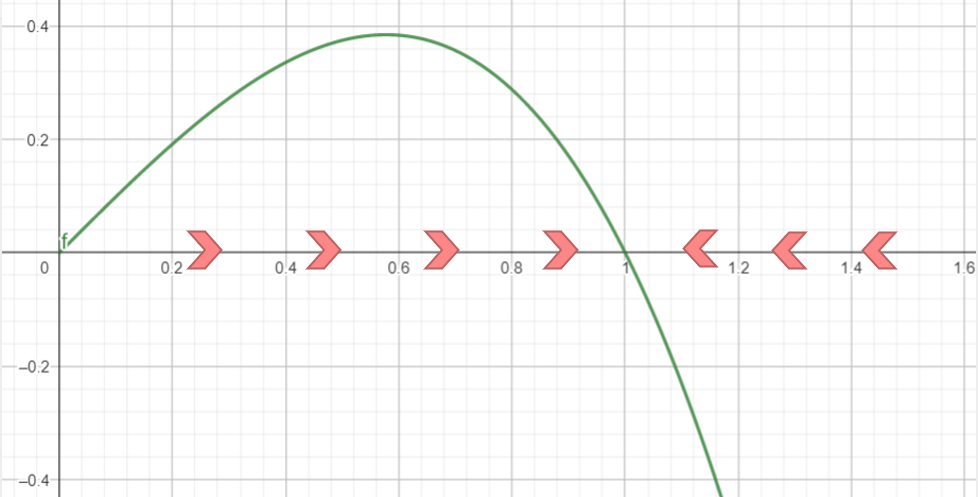
\includegraphics[width=14cm]{rej1.png}
	\caption{Plano fase de \eqref{eq:drsis1}.}
\end{figure}\\


Por otro lado para \eqref{eq:dthetasis1} la solución es $\theta(t)=t+\theta_0$,
donde $\theta_0=\theta(0)$.\\

Las soluciones del sistema \eqref{eq:sis1} convergen a puntos sobre la
circunferencia centrada en el origen de radio $1$.\\

Resolvamos el problema de forma analítica.\\

La ecuación \eqref{eq:drsis1} es separable
$$\int\frac{dr}{r(1-r^2)}=\int dt$$
integramos por fracciones parciales

$$\int\frac{dr}{r(1-r^2)}=\int\frac{dr}{r}-\int\frac{dr}{2(r+1)}-\int\frac{dr}{2(r-1)}$$
$$=\ln |r|-\frac{1}{2}\ln|r+1|-\frac{1}{2}\ln|r-1|+c_1$$

entonces
$$\ln |r|-\frac{1}{2}\ln|r+1|-\frac{1}{2}\ln|r-1|=t+c$$

desarrollamos logaritmos
$$\ln\left\lvert\frac{r^2}{r^2-1}\right\rvert=2t+c$$
$$\frac{r^2}{r^2-1}=ce^{2t}$$

$$r^2=\frac{e^{2t}}{c+e^{2t}}$$

Como $r\geq 0$
$$r=\frac{e^t}{\sqrt{c+e^{2t}}}$$
Aplicamos la condición inicial $r(0)=r_0$.\\
\\Las soluciones en coordenadas polares son:
\begin{equation}\label{eq: rsis1}
	r(t)=\frac{e^t}{\sqrt{\frac{1}{r_0^2}-1+e^{2t}}}
\end{equation}
\begin{equation}\label{eq: thetasis1}
	\theta(t)=t+\theta_0
\end{equation}
Dejaremos nuestra solución en coordenadas polares para realizar el siguiente
análisis del comportamiento asintótico.\\
\begin{enumerate}
	\item Si $r_0=1$ tenemos las ecuaciones
	      $$r(t)=1$$
	      $$\theta(t)=t+\theta_0$$
	\item Por otro lado, si $r_0>1$.
	      $$\lim_{t\to\infty}r(t)=\lim_{t\to\infty}\frac{e^t}{\sqrt{\frac{1}{r_0^2}-1+e^{2t}}}=1$$
	      $$\lim_{t\to-\infty}r(t)=\lim_{t\to-\infty}\frac{e^t}{\sqrt{\frac{1}{r_0^2}-1+e^{2t}}}=\infty$$
	\item Para $0<r_0<1$.
	      $$\lim_{t\to\infty}r(t)=\lim_{t\to\infty}\frac{e^t}{\sqrt{\frac{1}{r_0^2}-1+e^{2t}}}=1$$
	      $$\lim_{t\to-\infty}r(t)=\lim_{t\to-\infty}\frac{e^t}{\sqrt{\frac{1}{r_0^2}-1+e^{2t}}}=0$$
\end{enumerate}


Las trayectorias convergen a la circunferencia con centro en el origen
y de radio  $1$.\\

¿Qué significa que las trayectorias convergen a la circunferencia de centrada en el origen y de radio $1$?

\begin{definition} [Punto $\omega$ límite]
	Decimos que $\vec{z}\in\mathbb{R}^2$ es un punto $\omega$-límite
	de $\vec{x}_0\in\mathbb{R}^2$ si existe sucesión creciente de
	tiempos $\{t_n\}_{n\in\mathbb{N}}$
	con $t_n \to\infty$ cuando $n\to \infty$ tal que:
	$$\lim_{n\to\infty}\varphi^{t_n}(\vec{x}_0)=\vec{z}$$
\end{definition}

Regresemos las soluciones \eqref{eq: rsis1} y \eqref{eq: thetasis1} a
coordenadas cartesianas, con \eqref{eq:xpolar} y \eqref{eq:ypolar}.
\begin{equation}\label{eq: xsis1}
	x(t)=\frac{e^t\cos(t+\theta_0)}{\sqrt{\frac{1}{r_0^2}-1+e^{2t}}}
\end{equation}
\begin{equation}\label{eq: ysis1}
	y(t)=\frac{e^t\sin(t+\theta_0)}{\sqrt{\frac{1}{r_0^2}-1+e^{2t}}}
\end{equation}


\begin{figure}[h]
	\centering
	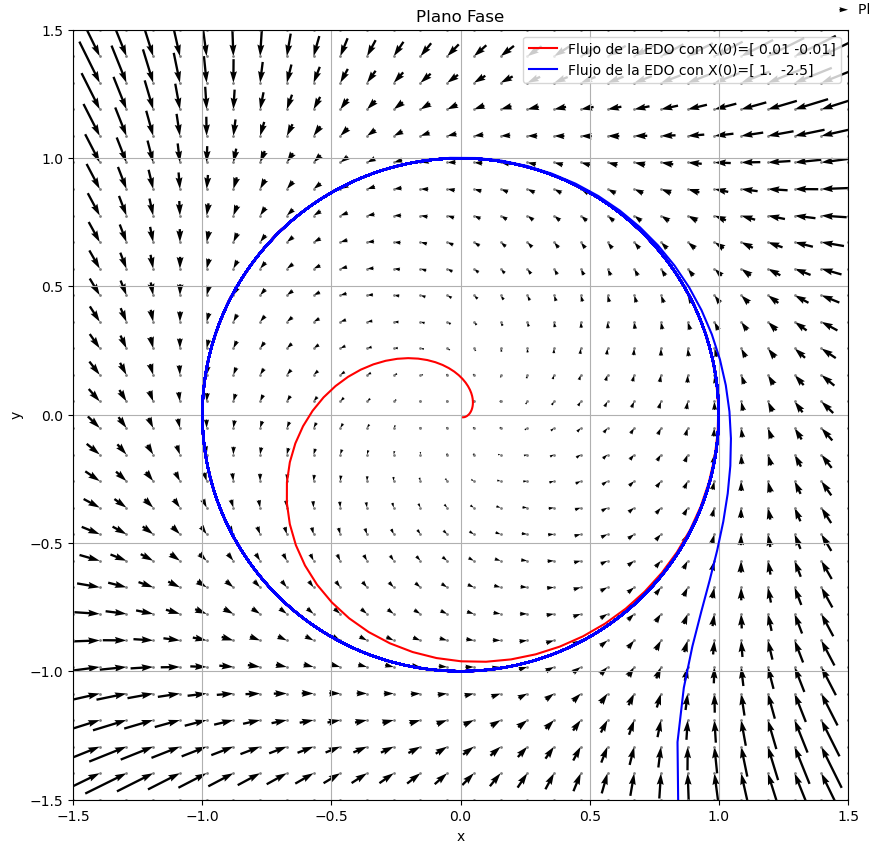
\includegraphics[width=13cm]{planofase1.png}
	\caption{Plano fase del sistema \eqref{eq:sis1}.}
\end{figure}

Tomemos la trayectoria en el plano fase de \eqref{eq:sis1} que pasa por el punto
$(x_0,y_0)$, entonces existe $\theta_0=\arctan(\frac{y_0}{x_0})\in[0,2\pi]$.
La trayectoria que pasa por $(x_0,y_0)$ está dada por las ecuaciones $\eqref{eq: xsis1}$ y
$\eqref{eq: ysis1}$ donde $x_0=x(0)$ y $y_0=y(0)$.\\
\\Tomemos un punto en la circunferencia centrada en el origen con radio $1$,
supongamos que
en coordenadas polares tiene un álgulo $0<\alpha_0<2\pi$, veamos que es punto $\omega$ límite, para eso podemos definir
$\{t_n=2\pi n+\alpha_0-\theta_0\}_{n\in \mathbb{N}}$, entonces
$$\lim_{n\to\infty}x(t_n)=\cos(\alpha_0)$$
$$\lim_{n\to\infty}y(t_n)=\sin(\alpha_0)$$
en efecto el punto $(\cos(\alpha_0),\sin(\alpha_0))$ es un punto $\omega$ límite, esto
quiere decir que para cada punto de la circunferencia podemos encontrar
una sucesión de tiempos $\{t_n\}_{n\in \mathbb{N}}$ con $t_n\to\infty$ tal que la
trayectoria converge a ese punto de la circunferencia, es decir cualquier punto que se encuentra en la
circunferencia centrada en el origen y de radio $1$ es un punto $\omega$ límite de $(x_0,y_0)$,
entonces diremos que esta circunferencia es un conjunto $\omega$ límite de $(x_0,y_0)$, donde
el conjunto $\omega$ límite se define como

$$\omega(\vec{X}_0)=\{\vec{z}\in\mathbb{R}^2\mid\vec{z} \text{  es  } \omega\text{-límite de  } \vec{X}_0\}.$$


Además, notemos que para $\{t_n=2\pi n+\alpha_0-\theta_0\}_{n\in \mathbb{N}}$,
la sucesión $\{(x(t_n),y(t_n))\}_{n\in\mathbb{N}}$ es una sucesión
de puntos convergente tal que sus puntos son colineales sobre la recta
$L=\{(x,y)\in\mathbb{R}^2\mid y=\tan(\alpha_0)x \}$. Las intersecciones de las trayectorias
son los valores de la sucesión colineal.\\

Modifiquemos el sistema \eqref{eq:drsis1}, a un sistema perturbado
con $0\leq\epsilon<1$.
\begin{equation}\label{eq: drmod}
	r'=r(1-r^2)+\epsilon r\cos(\theta)
\end{equation}
Veamos si existe $r_{max}$ tal que $r'<0$ y $r_{min}$ tal que $r'>0$.\\

Reescribimos \eqref{eq:drmod} como $r'=r(1-r^2+\epsilon \cos(\theta))$, como $r>0$,
entonces el signo de $r'$ depende de $1-r^2+\epsilon \cos(\theta)$.
Tenemos los siguientes casos:

\begin{enumerate}
	\item Si $1-r^2+\epsilon\cos(\theta)\leq 1-r^2+\epsilon<0$
	      entonces $\sqrt{1+\epsilon}<r_{max}$, por lo que para $r<r_{max}$ se tiene que $r'<0$.
	\item Por otro lado, si	$1-r^2+\epsilon\cos(\theta)>1-r^2-\epsilon>0$
	      entonces $\sqrt{1-\epsilon}>r_{min}$, por lo que para $r>r_{min}$ se tiene que $r'>0$.
\end{enumerate}

Las trayectorias que pasan por puntos en la circunferencia centrada
en el origen y con radio $r_{min}$
divergen del exterior de dicha circunferencia. Por otro lado,
las trayectorias que pasan por puntos en la circunferencia centrada
en el origen con radio $r_{max}$
convergen al interior del círculo.
A este segmento del plano lo llamamos región de atrapamiento.\\
\\Podemos intuir que debe existir
una curva cerrada en el interior, donde $r_{min}<r<r_{max}$, en la cual
las trayectorias convergen o alcanzan el equilibrio, de manera similar
a lo observado en el ejemplo
inicial, debido a su comportamiento. La idea de la existencia de una
curva cerrada de este tipo es lo que conocemos como ciclo límite.
\begin{figure}[h]
	\centering
	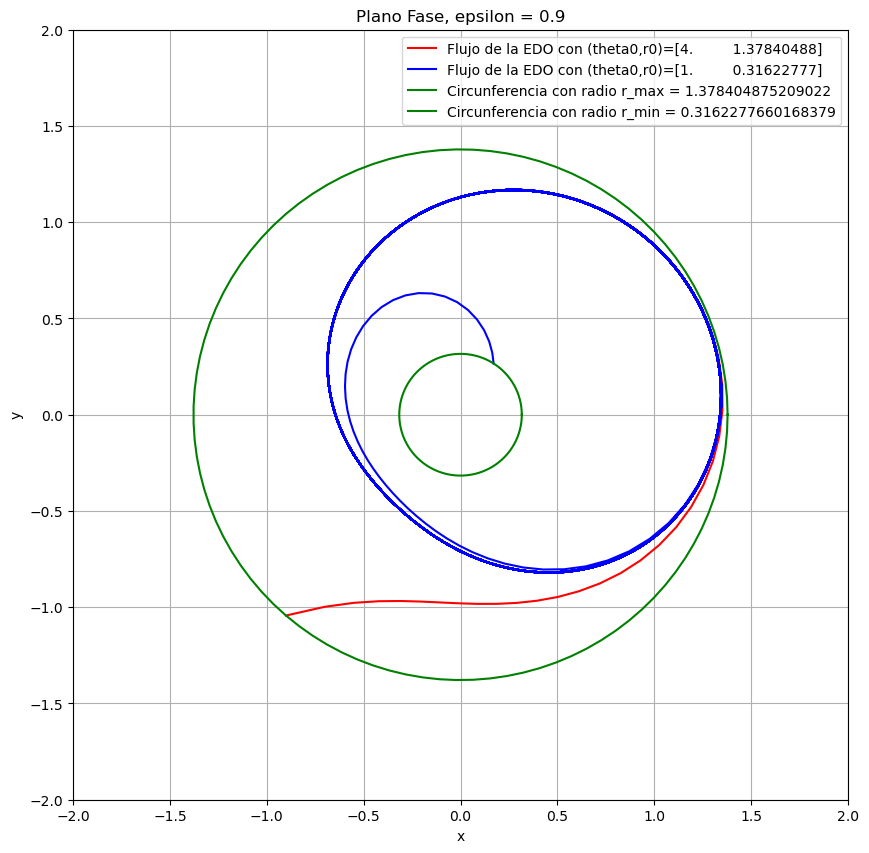
\includegraphics[width=13cm]{rminrmax.png}
	\caption{Plano fase del sistema con perturbación.}
\end{figure}

\newpage

\begin{definition}
	Definimos
	$$\varGamma_{\vec{x}}^{+}=\{\vec{y}=\varphi(t,\vec{x})\mid t>0\}$$
	$$\varGamma_{\vec{x}}^{-}=\{\vec{y}=\varphi(t,\vec{x})\mid t<0\}$$
	$$\varGamma_{\vec{x}}=\varGamma_{\vec{x}}^{+}\cup\varGamma_{\vec{x}}^{-}$$
\end{definition}

\begin{definition}
	Decimos que un conjunto $U$ es positivamente invariante si dado $\vec{x}\in U$ entonces  $\varGamma_{\vec{x}}^{+}\subset U$
\end{definition}

\begin{definition}
	Decimos que un conjunto $U$ es negativamente invariante si dado $\vec{x}\in U$ entonces  $\varGamma_{\vec{x}}^{-}\subset U$
\end{definition}

Notemos que esta sección del plano donde $r_{min}<r<r_{max}$ es positivamente invariante.
\newpage


\chapter{Implementación de la Teoría de promediación al problema 16 de Hilbert}

Vamos a implementar la teoría de promediación al 16 problema de Hilbert, vamos a descubir que información nos pueden dar sobre los ciclos límite de los sistemas, y cuales son sus limitaciones.\\

El sistema planar polinomial de grado $n$ lo podemos escribir como:

\begin{equation}\label{eq:P16H}
	\begin{matrix}
		x' =\displaystyle\large\sum_{0\leq i+j\leq n}a_{i,j}x^iy^j \\
		y' =\displaystyle\large\sum_{0\leq k+l\leq n}b_{k,l}x^ky^l 
	\end{matrix}
\end{equation}
con $i,j,k,l$ enteros no negativos. Vamos a transformar el sistema \eqref{eq:P16H} a coordenadas polares, primero sustituimos el sistema en \eqref{eq:drcart} y \eqref{eq:dthetacart}

\[
\begin{matrix}
	rr'=x\displaystyle\large\sum_{0\leq i+j\leq n}a_{i,j}x^iy^j +y \displaystyle\large\sum_{0\leq k+l\leq n}b_{k,l}x^ky^l \\
	r^2\theta' = x\displaystyle\large\sum_{0\leq k+l\leq n}b_{k,l}x^ky^l  -y\displaystyle\large\sum_{0\leq i+j\leq n}a_{i,j}x^iy^j 
\end{matrix}
\]

aplicamos el cambio de coordenadas \eqref{eq:xpolar} y \eqref{eq:ypolar}, obtenemos el sistema de ecuaciones en coordenadas polares:

\begin{equation}
	\begin{matrix}
		r'=\displaystyle\large\sum_{0\leq i+j\leq n}a_{i,j}r^{i+j}\cos^{i+1}(\theta)\sin^j(\theta) +\displaystyle\large\sum_{0\leq k+l\leq n}b_{k,l}r^{k+l}\cos^k(\theta)\sin^{l+1}(\theta) \\
		r\theta' = \displaystyle\large\sum_{0\leq k+l\leq n}b_{k,l}r^{k+l}\cos^{k+1}(\theta)\sin^l(\theta)  -\displaystyle\large\sum_{0\leq i+j\leq n}a_{i,j}r^{i+j}\cos^i(\theta)\sin^{j+1}(\theta) 
	\end{matrix}
\end{equation}

Vamos a analizar el sistema promediado $\widehat{r}'=\frac{1}{2\pi}\displaystyle\int_{0}^{2\pi}f(r,\theta)d\theta $

\end{document}